\documentclass[notitlepage]{report}
\usepackage{url}
\usepackage{hyperref}
\usepackage{graphicx}
\graphicspath{ {assets/} }
\usepackage{caption}

% discourage hyphenation
\tolerance=1
\emergencystretch=\maxdimen
\hyphenpenalty=10000
\hbadness=10000

% Subtract 1 from counters that are used
\renewcommand{\thesection}{\number\numexpr\value{section}\relax}
\renewcommand{\thesubsection}{\thesection.\number\numexpr\value{subsection}\relax}
\renewcommand{\thesubsubsection}{\thesubsection.\number\numexpr\value{subsubsection}\relax}
\setcounter{secnumdepth}{3}
\setcounter{chapter}{1}
\renewcommand\thefigure{\arabic{figure}}
\setcounter{figure}{0}
\setcounter{table}{0}

\title{Monero v7 Mining Pool Report}
% \date{May 2018}
\author{Josue Sneur \\
\textless\url{jsneur@gmail.com}\textgreater \\
(\url{https://github.com/jsneur})}

\begin{document}
\maketitle
\thispagestyle{empty}

\section*{Abstract}

This report applies to Monero mainnet version 7 (\verb/v7/) and showcases degraded privacy due to publicly-available metadata: mining pools' announced blocks and transactions.  Simple practices are presented which allow users and mining pools to proactively maintain privacy without disclosing less metadata.  Submissions are made to the blackball database and sample code is presented for scraping known spent outputs.

% \clearpage

\tableofcontents

\clearpage

\section{Introduction}
\setcounter{chapter}{1}

% \setcounter{page}{1} % Ignore the title/cover page; the Table of Contents and Introduction are page 1.

As of Monero version 7 (\verb/v7/, which began at block height 1546000,) a majority of the Monero hashrate is attributable to particular mining pools.  There are at least seven or eight public pools with over 1\% of the total global hashrate.  These pools advertise various statistics---metadata---including the blocks that they have mined.  All but one pool also list the payouts that they have made to their miners.  The combination of output ownership and transaction authorship allow the true member of some ring signatures to be inferred beyond a reasonable doubt in some cases, degrading one of Monero's layers of privacy.

\subsection{Monero's privacy layers}

Monero provides stealth addresses, ring signatures, and Ring Confidential Transactions (RingCT) as privacy layers as of \verb/v7/.  These layers ensure that Monero transactions are unlinkable, untraceable, and opaque.  Stealth addresses provide unlinkability by encrypting the recipients of payments such that only the recipient of a Monero transaction can detect it as addressed to them, ring signatures provide untraceability by concealing the source of a payment such that any one of a number of ring members should be equally-plausible as the actual source of a Monero transaction, and Ring Confidential Transactions provide opaqueness by encrypting a payment's input and output amounts such that a third party cannot discern anything related to a transaction's amounts other than that it did not create new coins.

\subsection{Degraded untraceability of ring signatures due to poor mining pool practices}

Ring signatures should conceal the real source of a Monero transaction: there is no way to discern which ring member actually made the transaction without additional information.  Unfortunately, metadata announcements due to poor mining pool practices such as blockchain forks and routine statistics advertisements can provide enough additional information to discern which ring member is the actual source of a transaction.

Blockchain forks have the potential to degrade the untraceability of ring signatures when key images are reused on both sides of a blockchain fork without taking advantage of any of the tools provided by Monero's \verb/v7/ upgrade.  Key images may be safely (at least privately) reused across blockchain forks if care is taken to construct identical rings on both sides of the fork (a process which is outside of the scope of this report but is described in detail \href{https://monero.stackexchange.com/questions/7826/how-can-individuals-safeguard-themselves-and-the-community-against-a-key-reusing}{here}.\footnote{``'How can individuals safeguard themselves and the community against a key reusing fork?'' https://monero.stackexchange.com/questions/7826/how-can-individuals-safeguard-themselves-and-the-community-against-a-key-reusing})  If users send funds on both sids of the fork without any such precautions, however, then they will inadvertently produce two rings that share only one member in common, thus identifying the common member as the real source of both transactions.  Such outputs are identified as ``known spent.''

Before any blockchain forks had incentivized key image reuse, mining pools were inadvertently revealing the real source of some payments \textit{via} the statistics that they advertise.  Mining pools announce their block.  When they later announce a transaction that uses one of their blocks' outputs as a ring signature member, it is most likely that their output is the real one and thus known spent.

By identifying an output as real in one transaction, its suitability as a decoy is degraded elsewhere, reducing the effective ring size of other users' ring signatures when included in rings after they are revealed to be known spent.

\subsection{Monero version 7's countermeasures against mining pool privacy degradations}

Several tools were provided by the Monero \verb/v7/ upgrade that allow users to avoid or mitigate of the above potential degradations to their privacy outlined previously.  For example, users can avoid including any known spent outputs in their own ring signatures by using what is known as the blackball database, which contains every known spent output.  This report presents additional submissions to the blackball database, including explanations of what metadata identifies the real member of a ring, where to collect it, and example code to scrape and analyze the metadata necessary for independent verification of these results.

\section{The State of the Hashrate}
\setcounter{chapter}{2}

As of \verb/v7/, a majority of the network hashrate is attributable to public mining pools.\footnote{See Figure \ref{fig:hashrate-distribution} from \url{http://minexmr.com/pools.html}; however, independent verification of this information is a topic for future work and is possible as long as mining pools publicly disclose either a reported hashrate or at least their found blocks.}  The top 8 public Monero pools (in descending order of hashrate) are: Nanopool, SupportXMR, mineXMR.com, Mining Pool Hub, F2Pool, MinerGate, DwarfPool, and MoneroHash.  These pools represent over 80\% of the combined global hashrate.  They all announce enough information to discern some outputs as known spent.\footnote{All of the pools announce their finds (blocks) and all but one (Nanopool) list all of their payments (transactions.)  Nanopool does not directly announce all of their payments, but still announces enough information to identify some outputs as spent, as detailed in section \ref{Nanopool}.  What portion of their total payments are attributable is not known at this time and is a topic for future work.}

\begin{figure}[h]
\centering
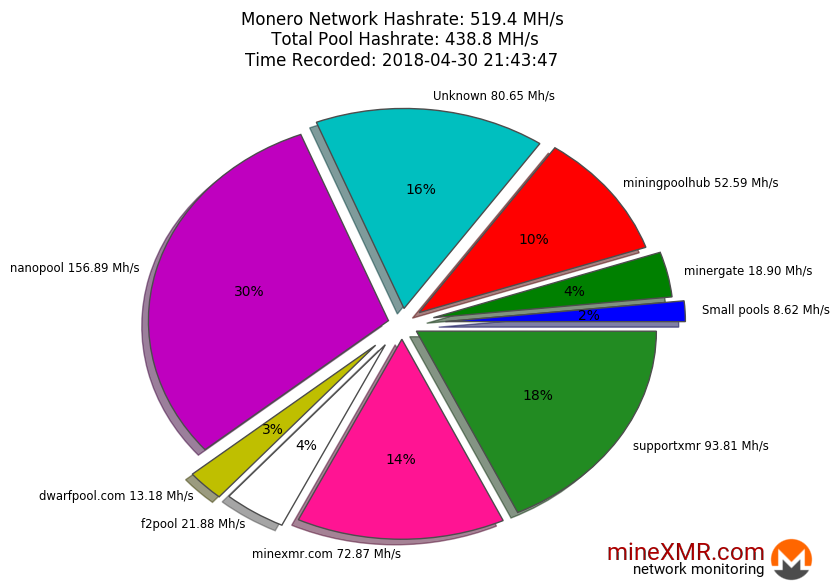
\includegraphics[width=\textwidth]{global-monero-mining-network-hashrate-distribution-2018-04-30}
\captionsetup{labelformat=empty}
\caption{Global Monero Mining Network Hashrate Distribution}
\label{fig:hashrate-distribution}
\end{figure}

\subsection{Software centralization}

TODO: List the most common mining pool stratum servers and GUIs and how code reuse enabled scraping of the data used to prepare this report.  \textit{Thanks, poolui!}

% Generated by https://www.tablesgenerator.com/markdown_tables

\begin{table}[h]
\centering
\caption{Top 8 Public Monero Mining Pools}
\begin{tabular}{lll}
Pool name       & API format                  & API endpoint                          \\ 
Nanopool        & \verb/nanopool/             & \url{https://api.nanopool.org/v1/xmr} \\ 
SupportXMR      & \verb/poolui/               & \url{https://supportxmr.com/api}      \\ 
mineXMR.com     & \verb/node-cryptonote-pool/ & \url{https://p5.minexmr.com}          \\ 
Mining Pool Hub &                             &                                       \\
F2Pool          &                             &                                       \\
MinerGate       &                             &                                       \\
DwarfPool       &                             &                                       \\
MoneroHash      &                             &                                 
\end{tabular}
\label{table:top-8-pools}
\end{table}

% TODO remake the chart above with overlays labelling distribution of software.

\section{Metadata collection}
\setcounter{chapter}{3}

Let $O$ be the set of a pool's outputs and $T$ be the set of a pool's transactions; if any of their outputs $o$ ($o \in O$) are used as a ring member in a later transaction $t$ ($t \in T$),) then that output $o$ is probably the real member of the ring signature: it is ``known spent.''

\subsection{Scrape mining pool APIs for blocks (coinbase outputs)}

All pool API formats make it easy to scrape mining pools for their blocks.  Suffix the ``API call'' column (where \verb/N/ is an integer) to the appropriate ``API endpoint'' column from table \ref{table:top-8-pools}.

\begin{table}[h]
\centering
\caption{Mining pool API endpoints for a mining pools' found blocks}
\begin{tabular}{lll}
Pool format     & Found blocks API           \\
poolui          & \verb|pool/blocks?limit=N| \\
nanopool        & \verb|pool/blocks/N|       \\
mineXMR.com     & \verb|stats|
\end{tabular}
\label{table:blocks-api}
\end{table}

% TODO example responses and explain parsing

\subsection{Scrape mining pool APIs for transactions}

All pool API formats make it easy to scrape mining pools for their transactions except for Nanopool.  Nanopool's scraping is the topic of section \ref{sec:nanopool}.  For all other API formats, just suffix the ``API call'' column to the appropriate their ``API endpoint'' column.

\begin{table}[h]
\centering
\caption{Mining pool API endpoints for transactions}
\begin{tabular}{lll}
Pool format     & Transaction history API      \\
poolui          & \verb|pool/payments?limit=N| \\
nanopool        & \textit{none}                \\ % Add API endpoint for payments to a particular address
mineXMR.com     & \textit{to do}
\end{tabular}
\label{table:transactions-api}
\end{table}

\subsubsection{Nanopool} \label{nanopool}

\section{Mitigation}

TODO: Pool operators: either announce less information *or* churn prior to paying out to miners.

\subsection{Blackball database submissions}

TODO: Describe the https://xmreuse.daemon.network API for querying blackball database submissions

\section{Future work}

\subsection{Maintenance of node-cryptonote-pool as node-monero-pool?}

\section{Conclusion}

\section{References}

\end{document}
